% Results and Evaluation

\chapter{نتایج و ارزیابی}\label{ch:5}
\section{مقدمه}\label{sec:5:1}
در این فصل دو روش \lr{KNN-LSTSVM} و \lr{RKNN-TSVM} به ترتیب در بخش‌های ‏\ref{sec:5:2} و ‏\ref{sec:5:3} به صورت جامع بررسی و ارزیابی می‌شود. این روش‌ها در دو بخش جداگانه مورد بررسی قرار گرفته‌اند. زیرا ایده و هدف اصلی این دو روش با یکدیگر متفاوت است. 
\begin{enumerate}
	\item هدف اصلی در روش \lr{KNN-LSTSVM} ضمن حفظ مزیت اصلی روش \lr{LSTSVM}، اضافه کردن گراف نزدیک‌ترین همسایه به منظور بهبود دقت این مدل است.
	\item 	روش \lr{RKNN-TSVM} با کمینه کردن ریسک ساختاری و شیوه جدید وزن‌دهی، دقت روش \lr{WLTSVM} را بهبود می‌دهد. با این حال در روش \lr{RKNN-TSVM}، افزایش سرعت آموزش هم مد نظر است.
\end{enumerate}

در ادامه عملکرد روش پیشنهادی از نظر دقت و سرعت روی مجموعه داده‌های مختلف سنجیده می‌شود.

\section{ارزیابی روش \lr{KNN-LSTSVM}}\label{sec:5:2}
ابتدا نحوه پیاده‌سازی و انتخاب پارامترهای بهینه توضیح داده شده است. سپس عملکرد روش \lr{KNN-LSTSVM} روی مجموعه داده‌های مصنوعی بررسی می‌شود. بطوریکه ناحیه تصمیم خطی و غیر خطی این روش در فضای دو بعدی نشان داده شده است. در آخر نتایج روی مجموعه داده‌های \lr{UCI} و \lr{NDC} مورد بحث قرار می‌گیرد.

\subsection{نحوه پیاده‌سازی و اجرای الگوریتم‌ها}\label{sec:5:2:1}
تمام روش‌ها در زبان برنامه‌نویسی پایتون\footnote{\lr{Python}}  \cite{ceder2010} پیاده‌سازی شده است. آزمایش‌ها روی یک کامپیوتر شخصی با پردازنده \lr{Core i7 6700K}، سیستم عامل \lr{Windows 8} و 32 گیگابایت حافظه صورت گرفته است. اعمال جبر خطی با کتابخانه \lr{NumPy} \cite{walt2011} انجام شده است. همچنین کتابخانه \lr{SciPy} \cite{jones2014} برای محاسبه فاصله و توابع آماری بکار گرفته شده است. همچنین الگوریتم بهینه‌سازی \lr{clipDCD} جهت بهبود سرعت اجرا، در \lr{Cython} \cite{behnel2011} پیاده‌سازی شده است.

دقت روش \lr{TSVM} و گسترش‌هایش به انتخاب پارامترهای بهینه بسیار وابسته است. بدین منظور جستجوی شبکه‌ای\footnote{\lr{Grid search}}  برای پیدا کردن پارامترهای بهینه استفاده می‌شود. همچنین تابع \lr{TSVM} را به عنوان تابع هسته  $k(x_i, x_j)=\exp({-\left\|x_i - x_j\right\|^2}/\gamma^2)$ اغلب بکار می‌گیرند. پارامترهای خطا در روش‌های \lr{TSVM}، \lr{WLTSVM}، \lr{LSTSVM} و \lr{KNN-LSTSVM} از مجموعه  $\{2^i \mid i=-10, -9, \dots, 9, 10\}$ انتخاب شده است.  پارامتر تابع هسته $\gamma$  نیز از مجموعه  $\{2^i \mid i=-15, -14, \dots, 5\}$ تعیین می‌شود. تعداد نزدیک‌ترین همسایه  $k$ از مجموعه  $\{2,3, \dots, 10\}$ انتخاب می‌گردد.

\section{مجموعه داده مصنوعی}\label{sec:5:2:2}
به منظور نشان دادن برتری روش \lr{KNN-LSTSVM} نسبت به روش \lr{LSTSVM} به صورت هندسی، آزمایش روی مجموعه داده \lr{Ripley}  \cite{ripley2007} و \lr{Checkerboard} \cite{ho1996} انجام گرفته است که به ترتیب شامل 250 و 1000 نمونه آموزشی هستند. شکل ‏\ref{fig:LSTSVM-vs-KNN-LSTSVM-R} و شکل \ref{fig:LSTSVM-vs-KNN-LSTSVM-C} عملکرد و ناحیه تصمیم روش \lr{LS-TSVM} و \lr{KNN-LSTSVM} را به ترتیب برای روی مجموعه داده \lr{Ripley} و \lr{Checkerboard} نشان می‌دهد.

همانطور که در شکل ‏\ref{fig:LSTSVM-vs-KNN-LSTSVM-R} و شکل ‏\ref{fig:LSTSVM-vs-KNN-LSTSVM-C} نشان داده شده است، روش پیشنهادی \lr{KNN-LSTSVM} دقت بیشتر و ناحیه تصمیم بهتری دارد. بطوریکه تعداد نمونه‌های تست کمتری به طور اشتباه دسته‌بندی شده‌اند. به عبارت دیگر، تعمیم‌پذیری روش \lr{KNN-LSTSVM} بیشتر است.

\begin{figure}[!t]
	\centering
	\subfloat[\lr{LSTSVM} (\lr{$C=2^{-10}, \gamma=2^{1}$})]{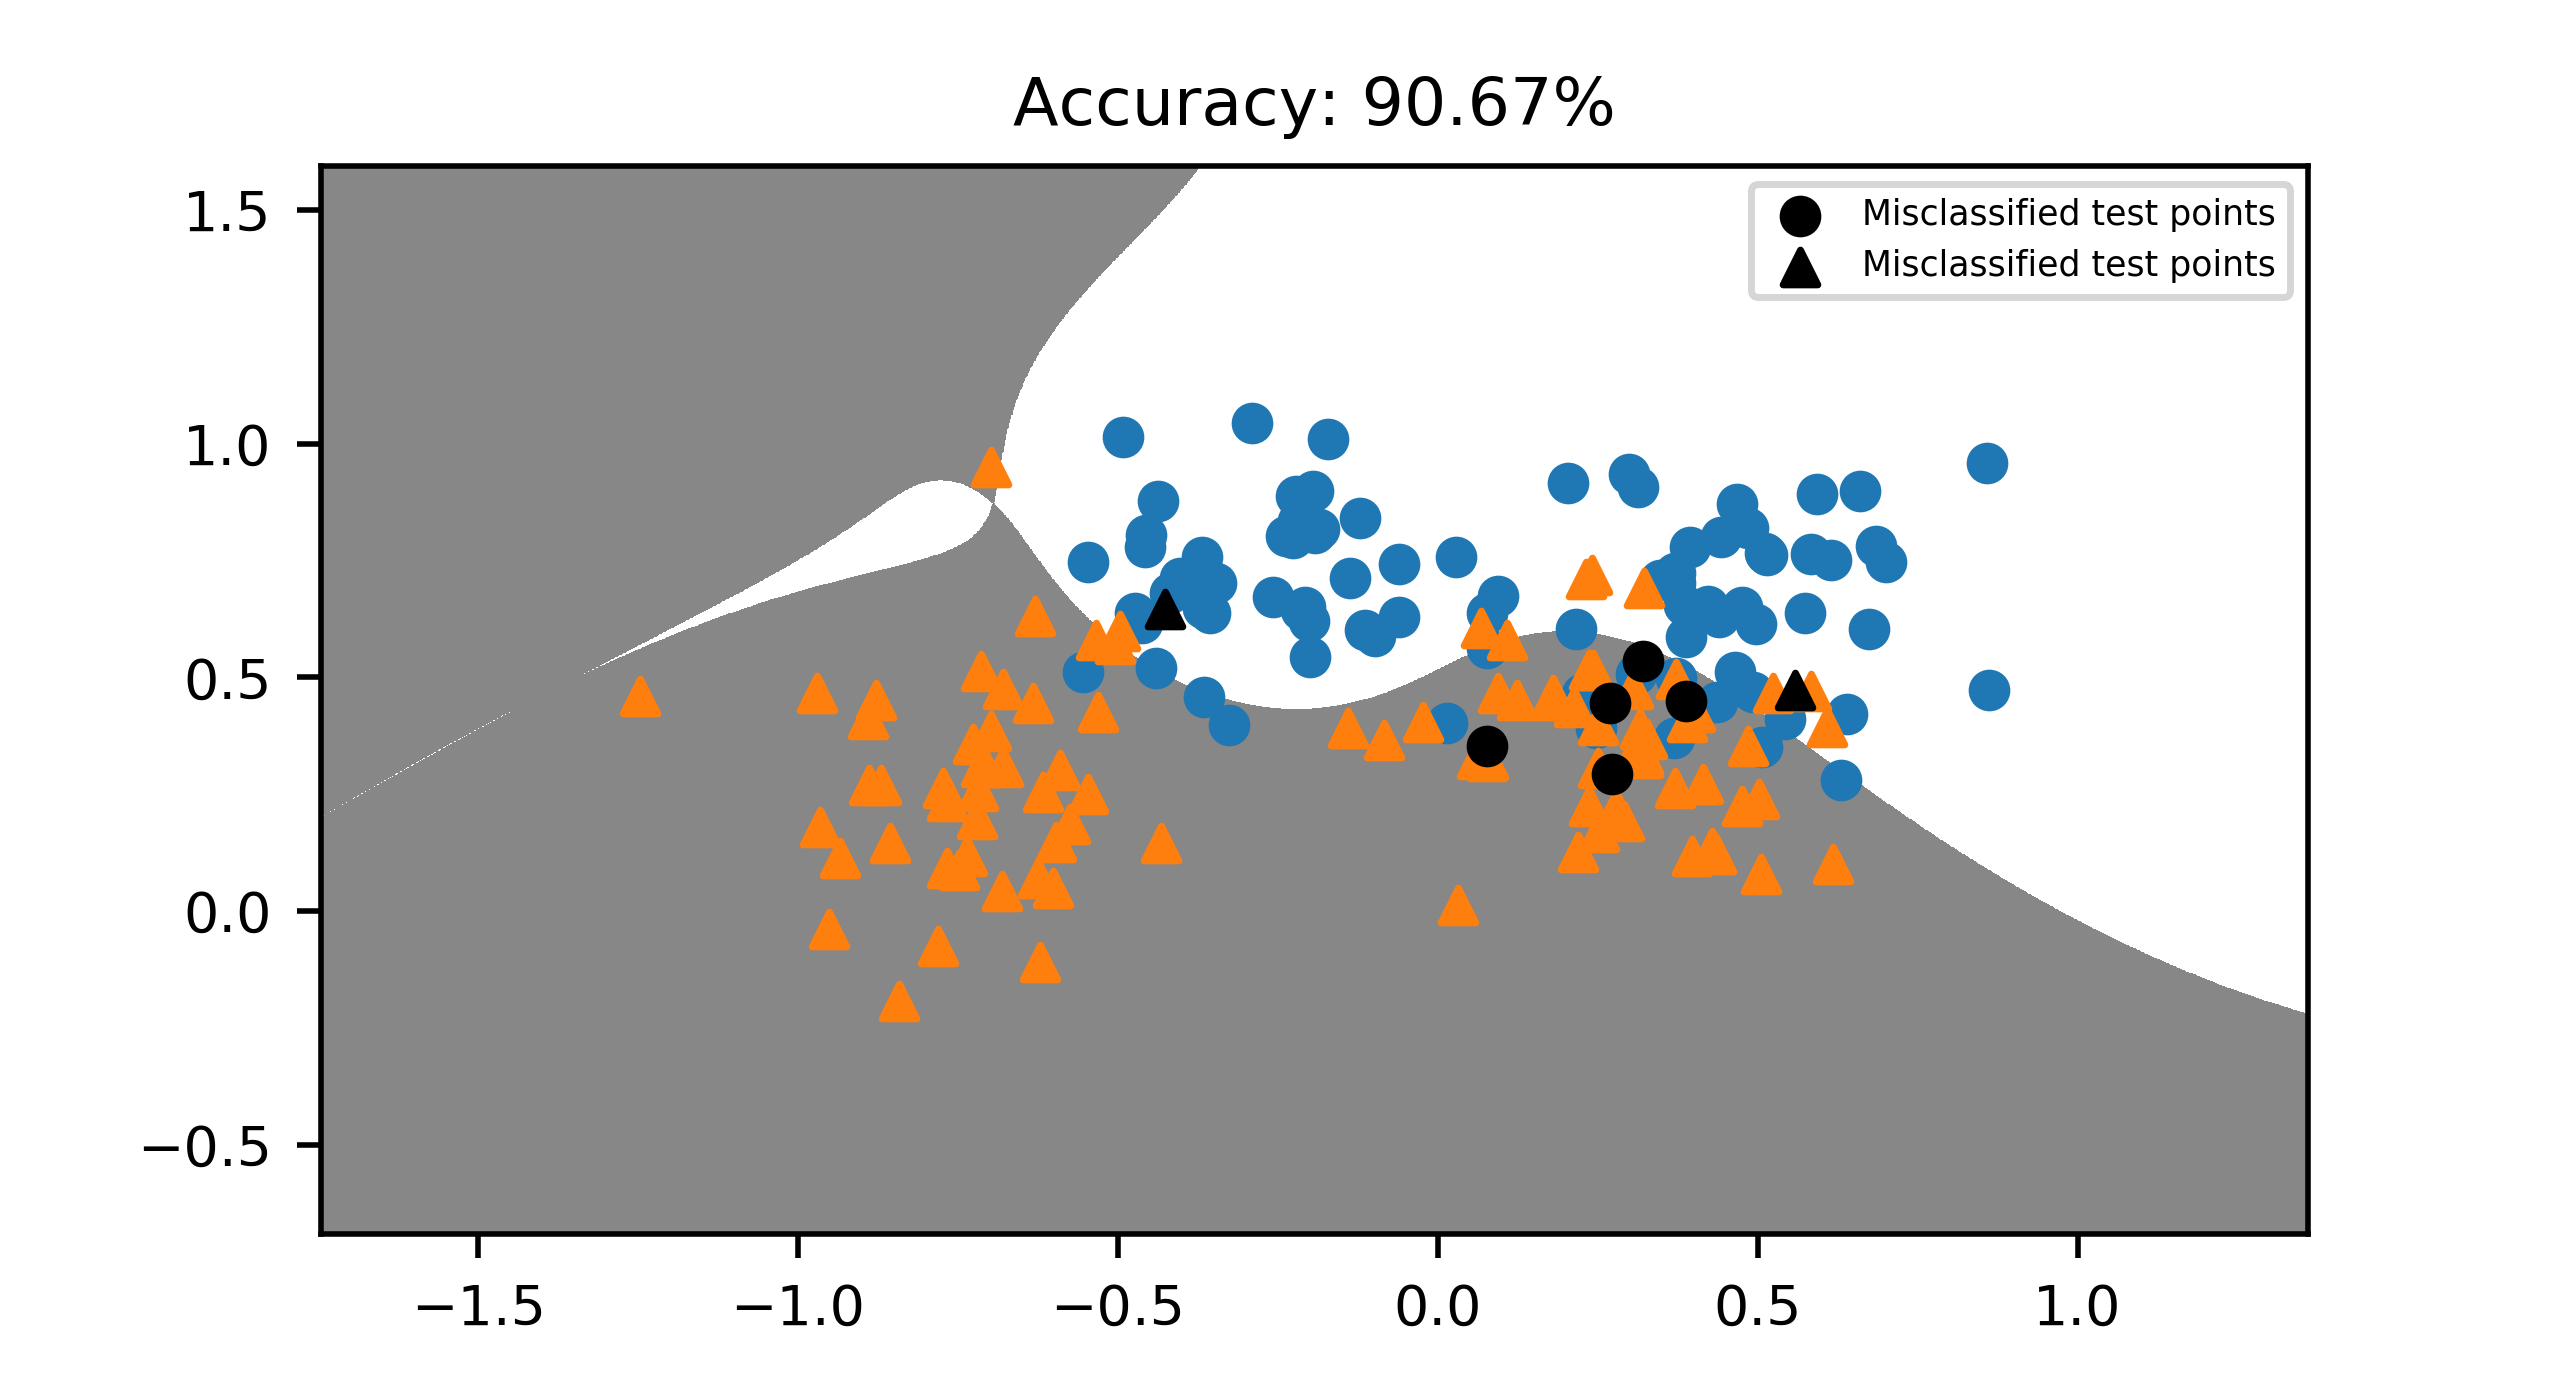
\includegraphics[width=0.5\textwidth]{LSTSVM-Ripley}}
	\subfloat[\lr{KNN-LSTSVM} \lr{($C=2^{-7}, k=6, \gamma=1$)}]{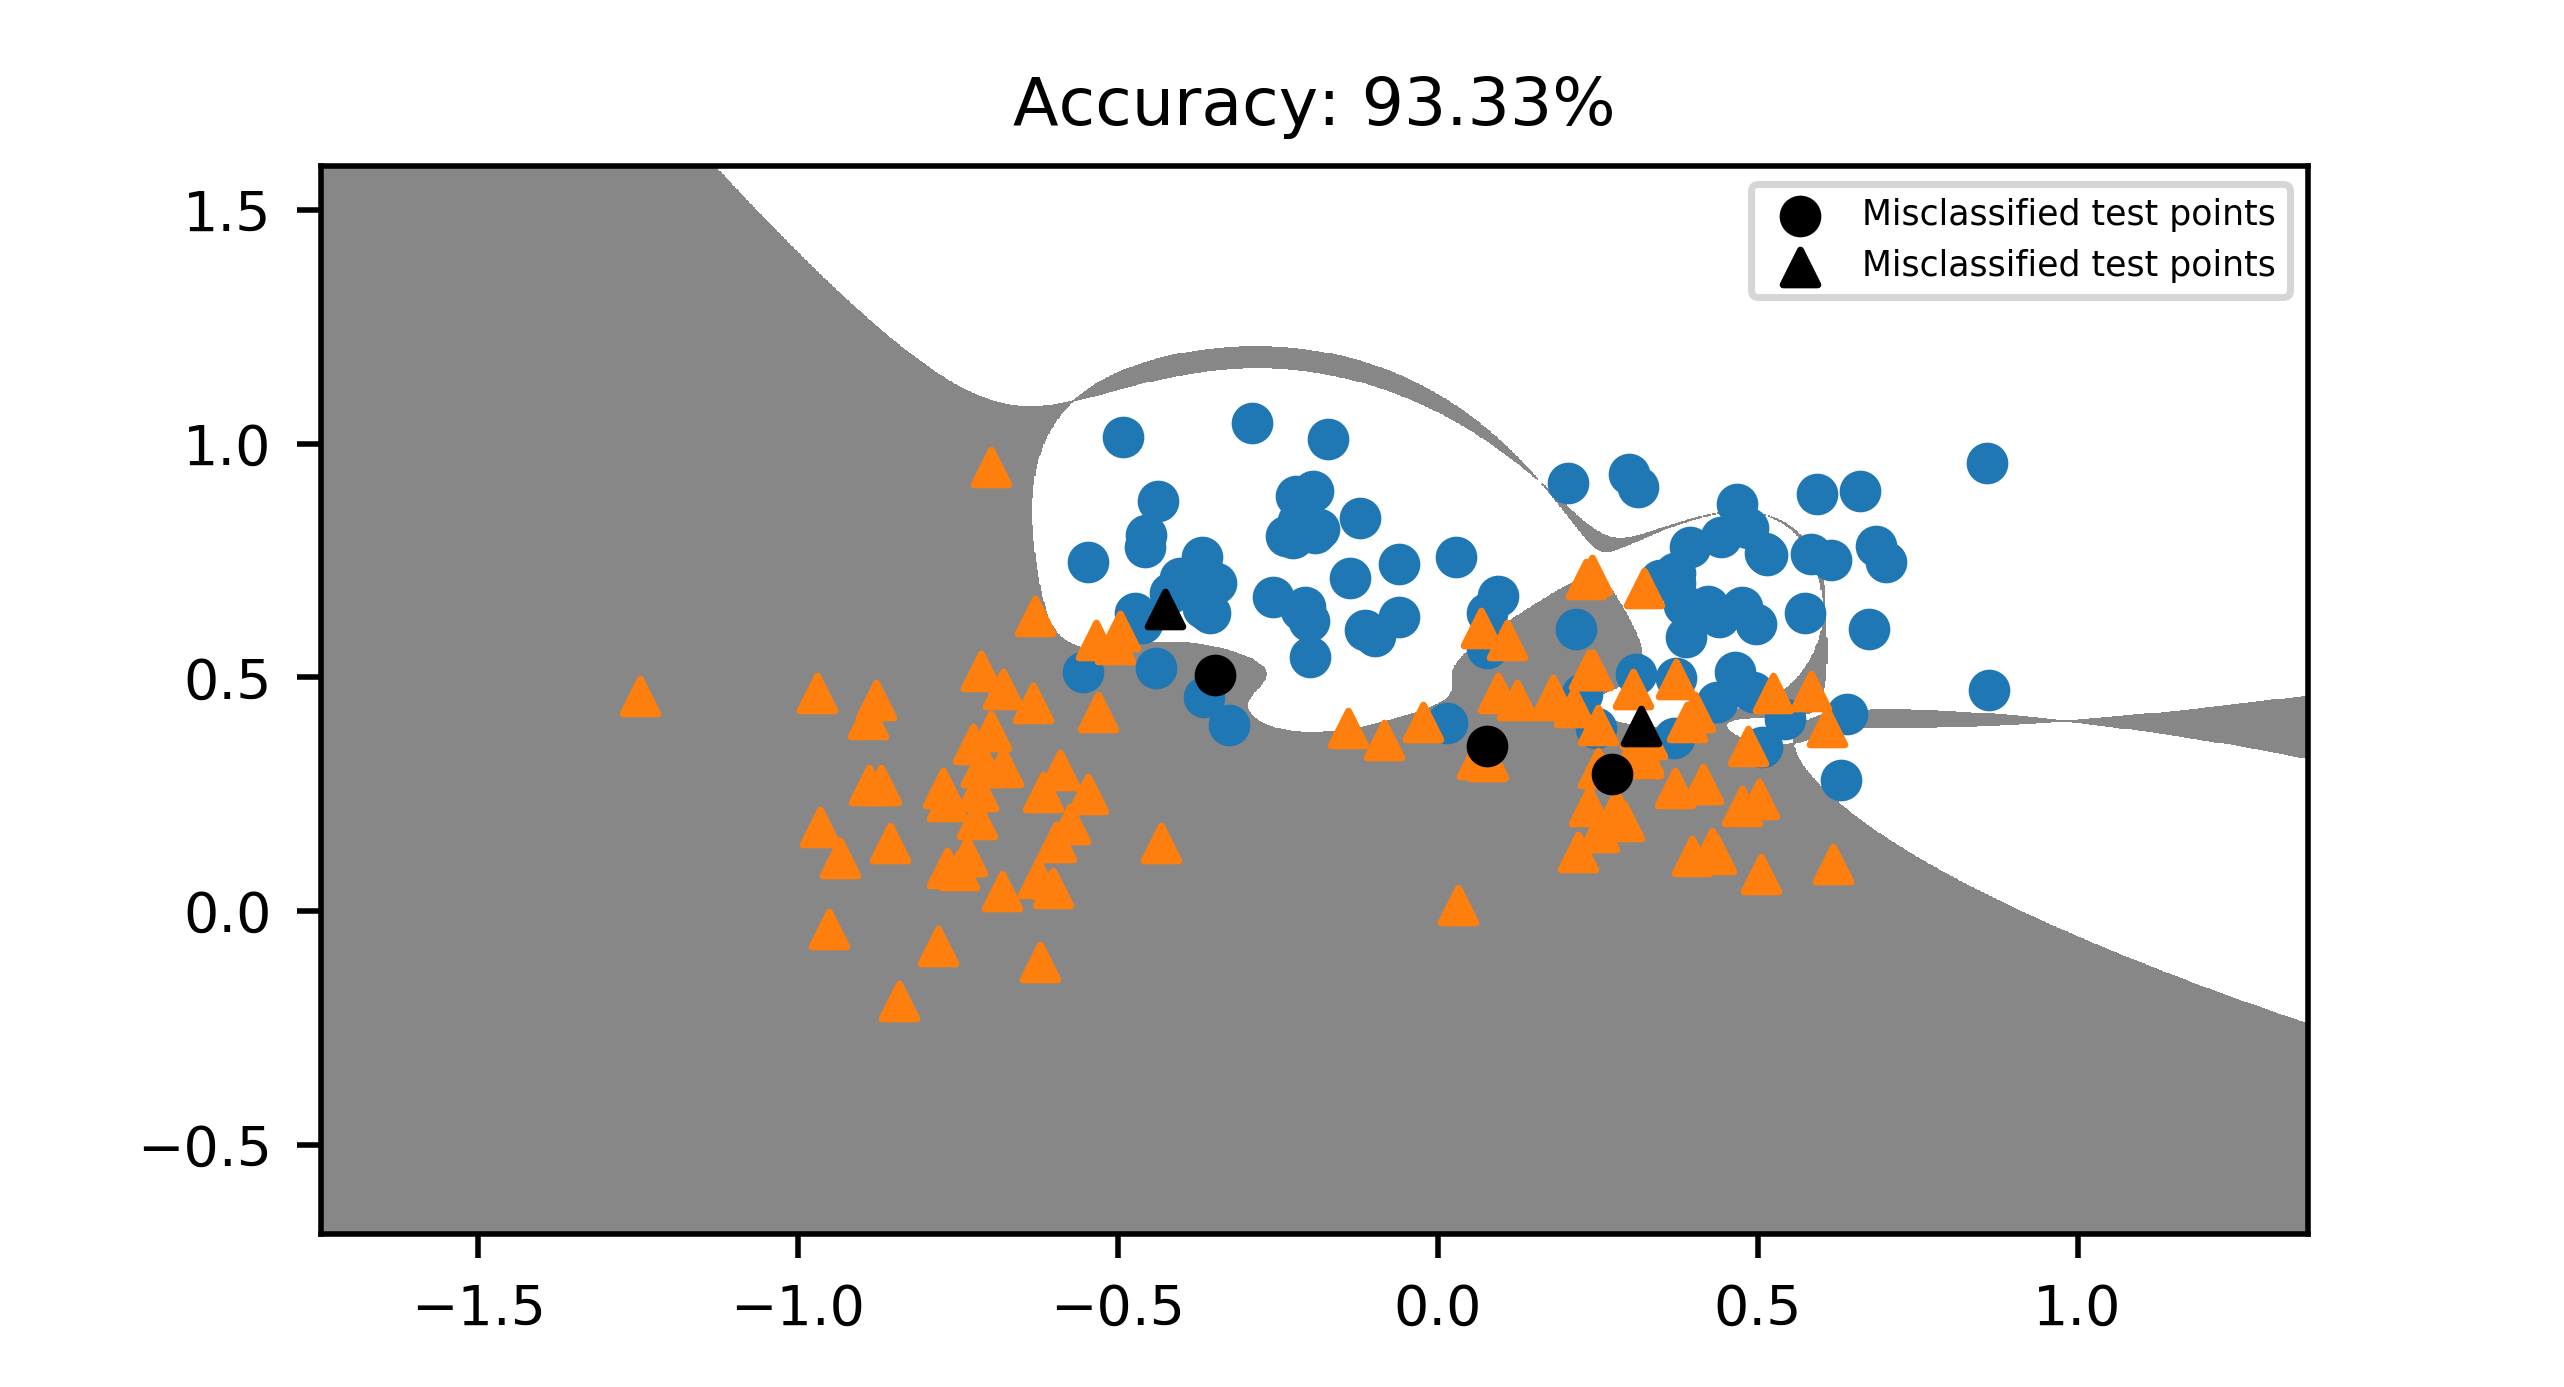
\includegraphics[width=0.5\textwidth]{KNN-LSTSVM-Ripley}}
	\caption{عملکرد و ناحیه تصمیم روش  \lr{LS-TSVM} و  \lr{KNN-LSTSVM} را برای روی داده  \lr{Ripley}}
		\label{fig:LSTSVM-vs-KNN-LSTSVM-R}
\end{figure}

\begin{figure}[!ht]
	\centering
	\subfloat[\lr{LSTSVM} (\lr{$C=2^{-10}, \gamma=2^{1}$})]{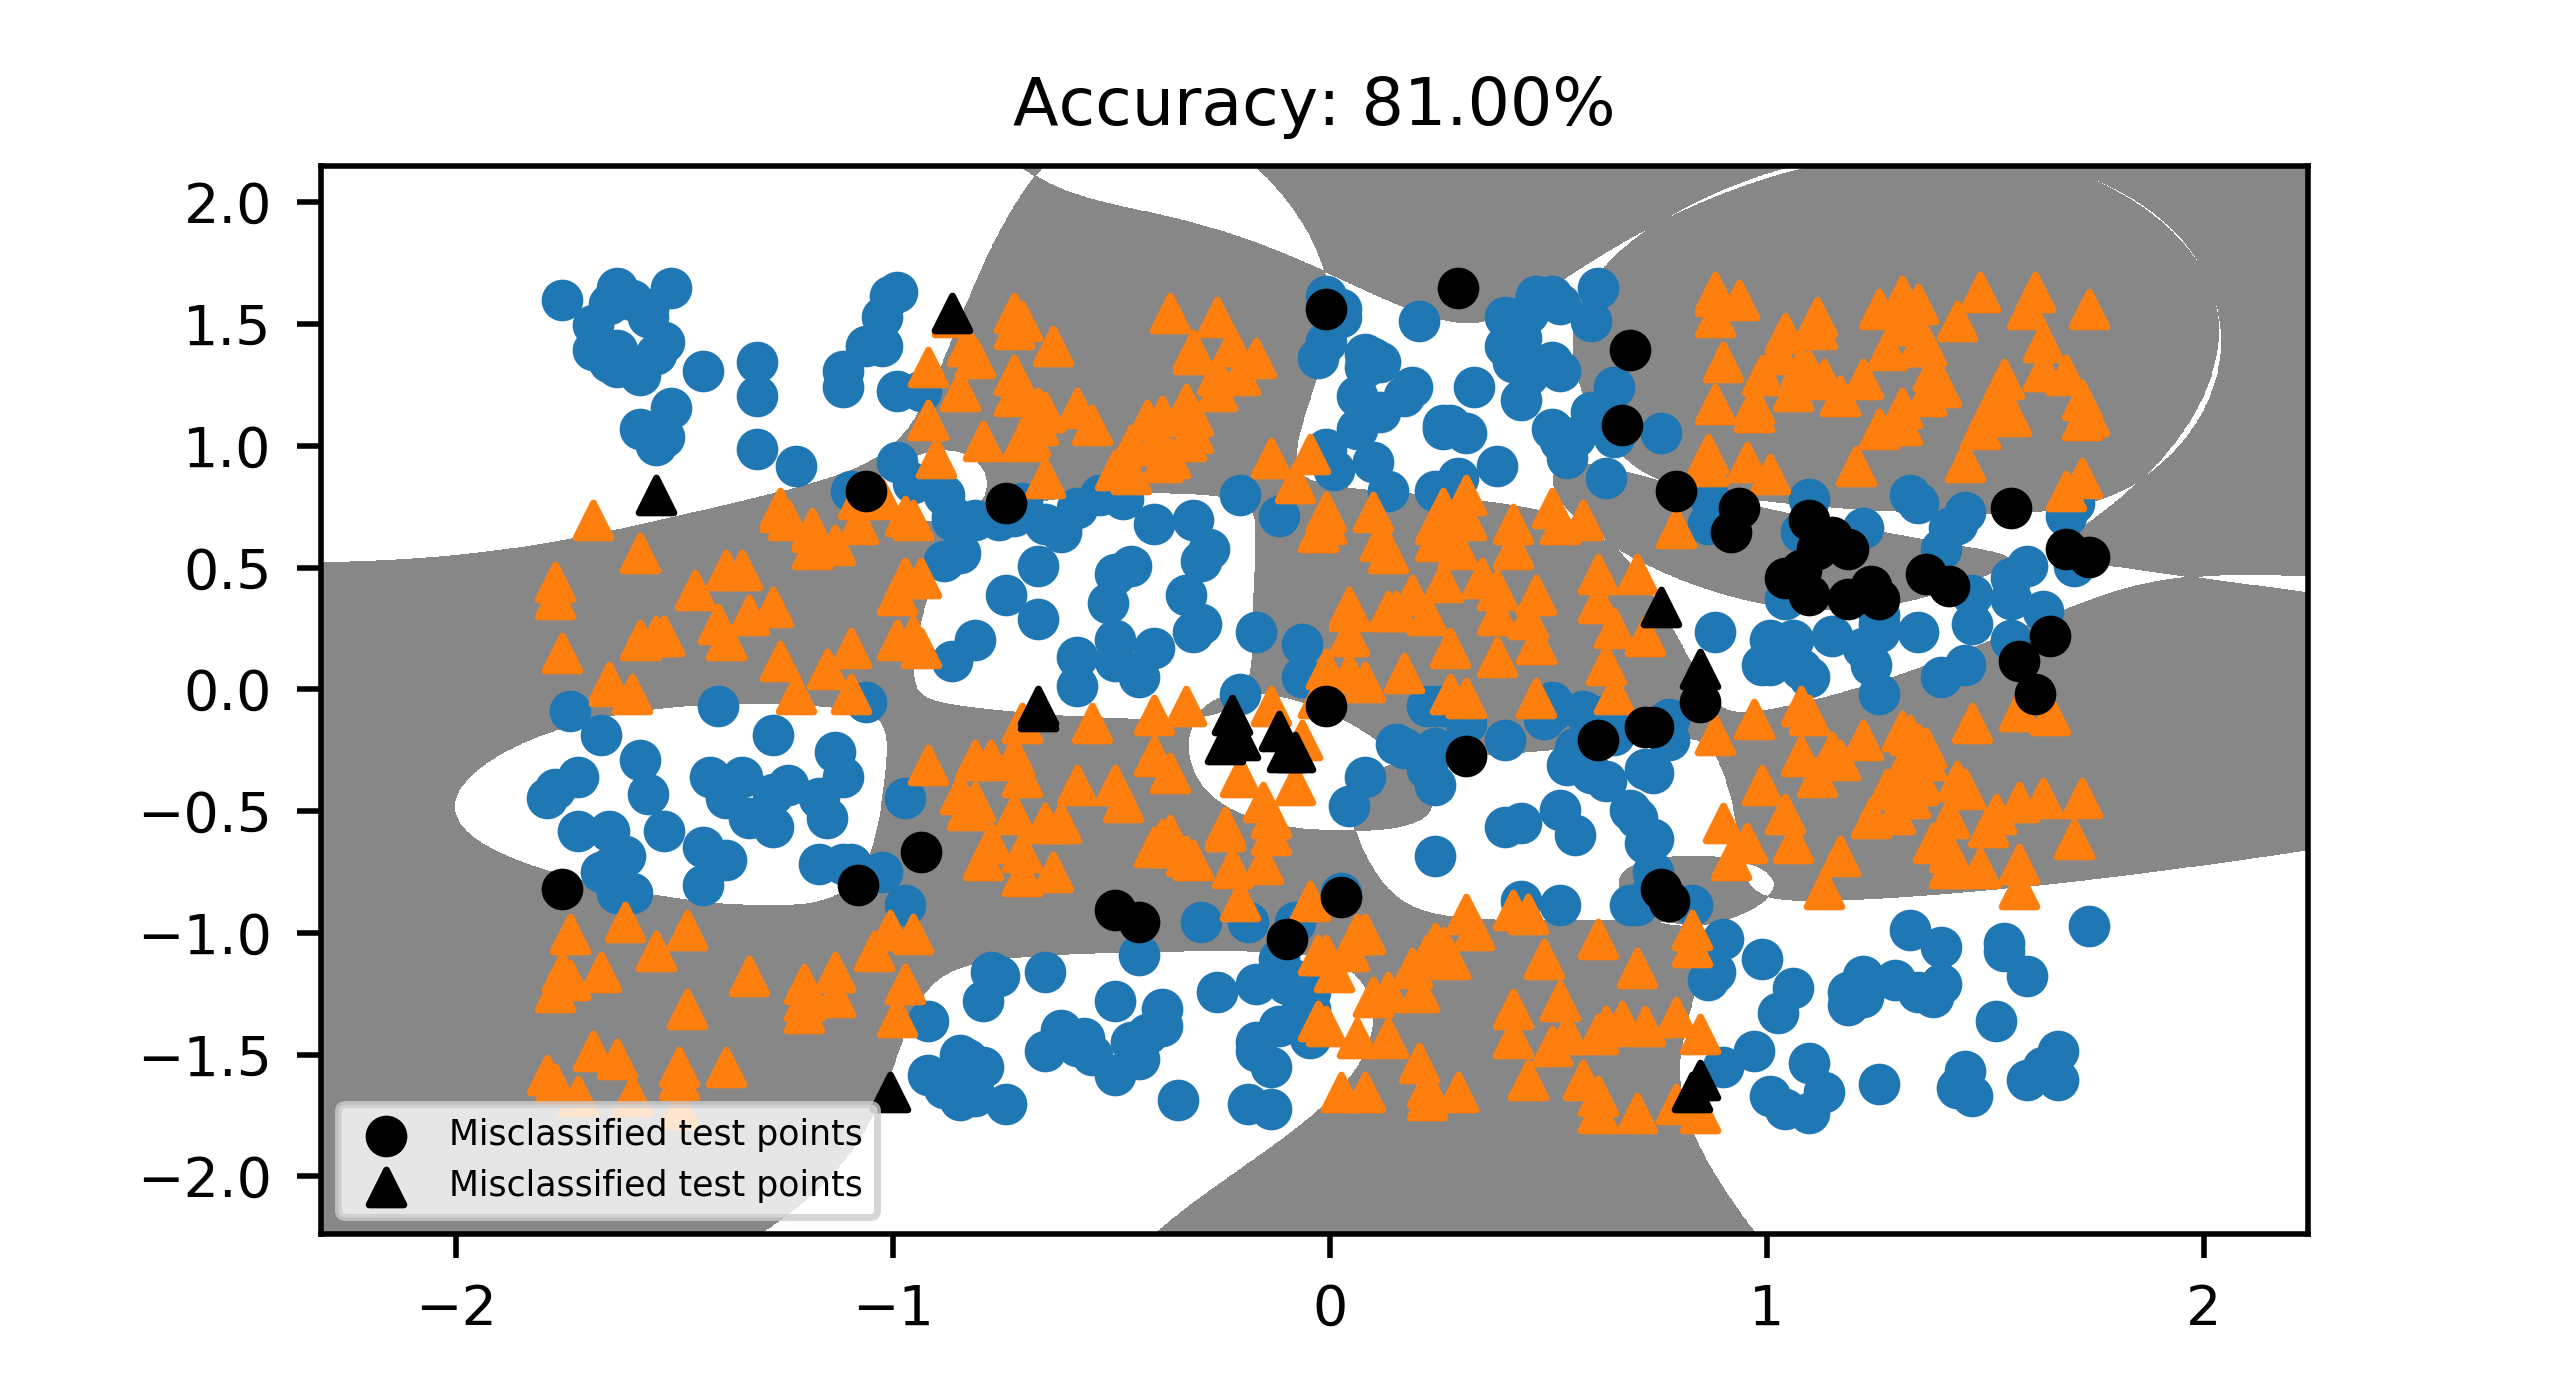
\includegraphics[width=0.5\textwidth]{LSTSVM-check}}
	\subfloat[\lr{KNN-LSTSVM} \lr{($C=2^{-10}, k=6, \gamma=2^{1}$)}]{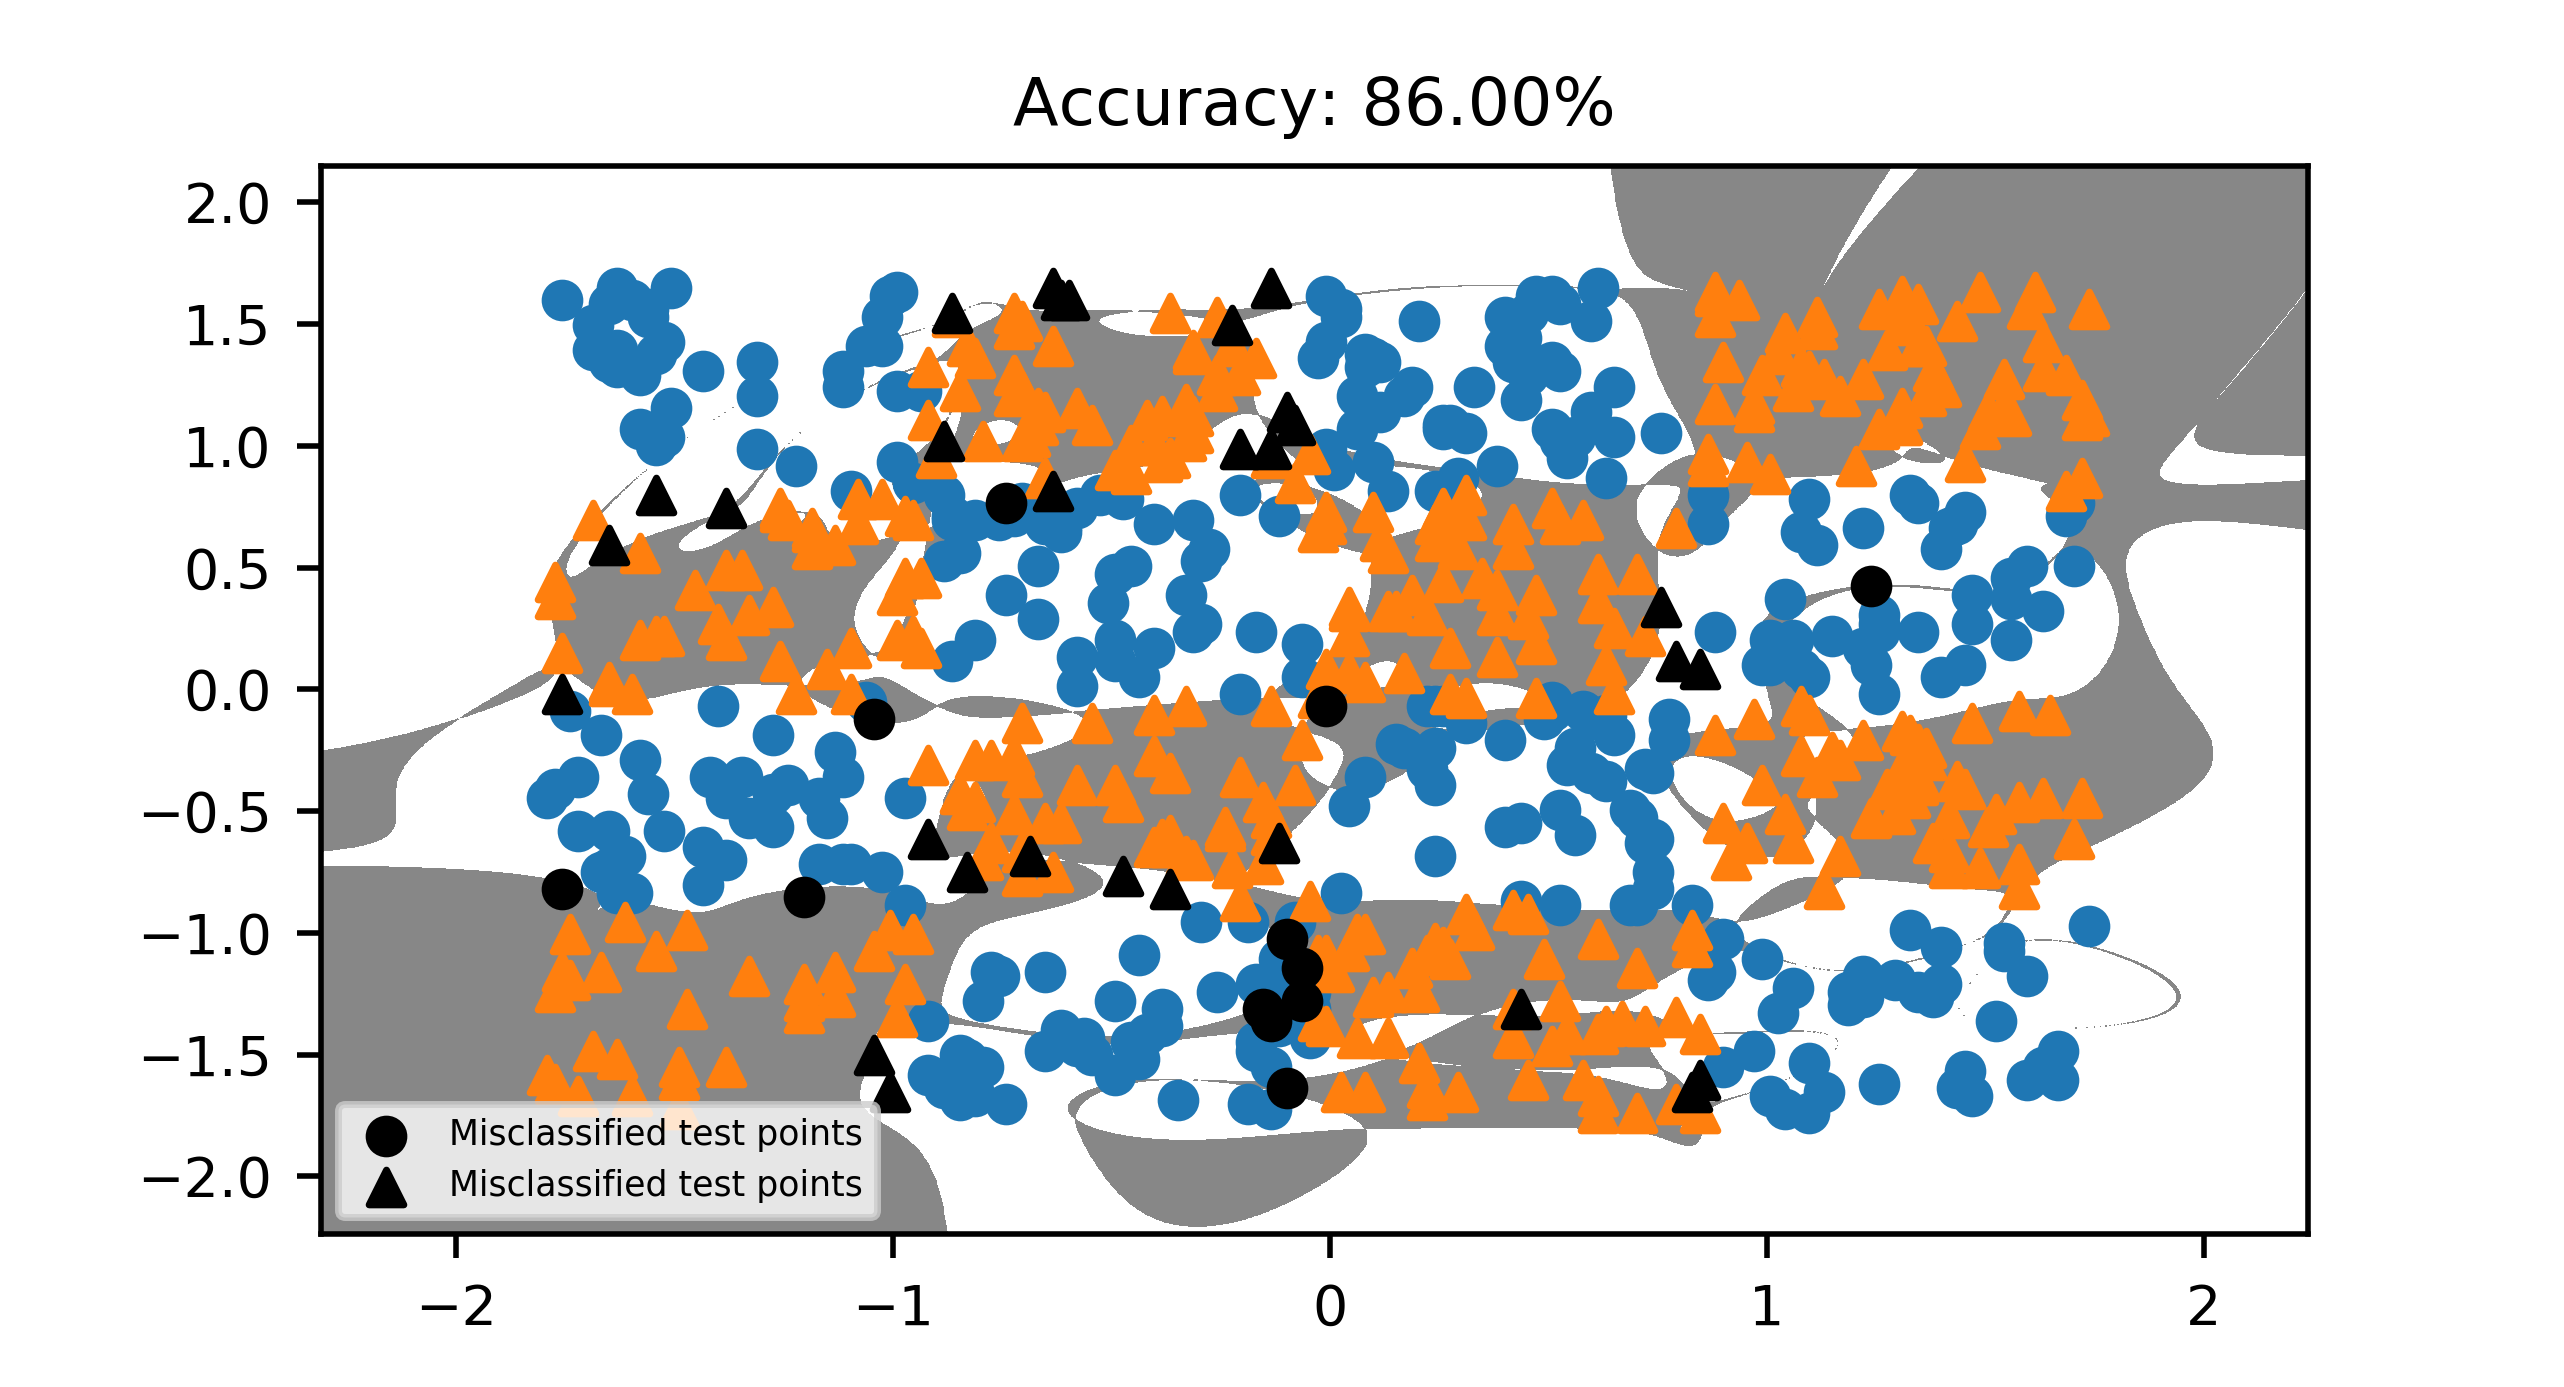
\includegraphics[width=0.5\textwidth]{KNN-LSTSVM-check}}
	\caption{عملکرد و ناحیه تصمیم روش  \lr{LS-TSVM} و  \lr{KNN-LSTSVM} را برای روی داده  \lr{Checkerboard}}
	\label{fig:LSTSVM-vs-KNN-LSTSVM-C}
\end{figure}

\newpage

\section{نتایج ارزیابی بر روی مجموعه داده \lr{UCI}}\label{sec:5:2:3}
در این زیر بخش، عملکرد روش \lr{KNN-LSTSVM} روی 14 مجموعه داده از مخرن  \lr{UCI}\footnote{\lr{https://archive.ics.uci.edu/ml/index.php}} ارزیابی و بررسی می‌شود. مشخصات این مجموعه داده‌ها در جدول \ref{tab:1} ذکر شده است.

\begin{table}[!t]
	\centering
	\caption{مشخصات مجموعه داده‌ها برای ارزیابی روش \lr{KNN-LSTSVM}}
	%\tabcolsep=0.11cm
	\begin{tabular}{l c c c c}
		\hline
		% after \\: \hline or \cline{col1-col2} \cline{col3-col4} ...
		مجموعه داده & تعداد نمونه‌ها & نمونه‌های مثبت & نمونه‌های منفی &تعداد ویژگی‌ها \\
		\hline
	\lr{{Austrailian}} & {690} & {307} & {383} & {14} \\
	\lr{{Bupa-Liver}} & {345} & {145} & {200} & {6} \\
	\lr{{Cleveland}} & {303} & {139} & {164} & {13} \\
	\lr{{Haber-Man}} & {306} & {225} & {81} & {3} \\
	\lr{{Heart-Statlog}} & {270} & {120} & {150} & {13} \\
	\lr{{Hepatits}} & {155} & {32} & {123} & {19} \\
	\lr{{Ionsphere}} & {351} & {225} & {126} & {34} \\
	\lr{{Monk3}} & {554} & {288} & {266} & {6} \\
	\lr{{Pima-Indian}} & {768} & {268} & {500} & {8} \\
	\lr{{Sonar}} & {208} & {97} & {111} & {60} \\
	\lr{{Titanic}} & {891} & {342} & {549} & {7} \\
	\lr{{Votes}} & {435} & {267} & {168} & {16} \\
	\lr{{Wdbc}} & {569} & {212} & {357} & {30} \\
	\lr{{Wpbc}} & {198} & {47} & {151} & {33} \\
		\hline
	\end{tabular}
	
	\label{tab:1}
\end{table}

دقت دسته‌بندی هر کدام از روش‌ها توسط معیار ارزیابی اعتبارسنج ضربدری  ۱۰تایی سنجیده می‌شود. بطوریکه نمونه‌های آموزشی به صورت تصادفی به 10 بخش تقیسم می‌شوند. یکی از این بخش‌ها به عنوان نمونه‌های تست در نظر گرفته می‌شود و سایر بخش‌ها برای آموزش دسته‌بند استفاده می‌گردد. این فرآیند 10 بار تکرار می‌شود تا زمانی که تمام بخش‌ها به عنوان نمونه تست استفاده شود \cite{bishop2006}.

جدول ‏5 2 میانگین و انحراف معیار دقت (به درصد) را برای دسته‌بندهای \lr{TSVM}، \lr{WLTSVM}، \lr{LSTSVM} و \lr{KNN-LSTSVM }نشان می‌دهد. همچنین زمان آموزش دسته‌بندها (به ثانیه) نیز در جدول ‏5 2 درج شده است. لازم به ذکر است که محاسبه گراف نزدیک‌ترین همسایه در زمان آموزش دسته‌بندهای \lr{WLTSVM} و \lr{KNN-LSTSVM} لحاظ شده است. $3.14$

\begin{table*}[!t]
	\centering
	\caption{مقایسه دقت و زمان آموزش دسته‌بندهای \lr{TSVM}، \lr{WLTSVM}،  \lr{LSTSVM} و \lr{KNN-LSTSVM}}
	\ra{1.3} % Space between rows
	\tabcolsep=0.13cm % Adjusts column width
	\begin{tabular}{p{2.1cm} p{1.85cm} p{1.1cm} c p{1.85cm} p{1.1cm} c p{1.85cm} p{1.1cm} c p{1.85cm} p{1.1cm}}
		\toprule
		
		% after \\: \hline or \cline{col1-col2} \cline{col3-col4} ...
		Datasets & \multicolumn{2}{c}{TSVM} && \multicolumn{2}{c}{WLTSVM} && \multicolumn{2}{c}{LSTSVM} && \multicolumn{2}{c}{KNN-LSTSVM} \\
		\cmidrule{2-3} \cmidrule{5-6} \cmidrule{8-9} \cmidrule{11-12}
		($m\times n$) & Accuracy(\%) & Time(s) && Accuracy(\%) & Time(s) && Accuracy(\%) & Time(s) && Accuracy(\%) & Time(s) \\
		& $(C_1, C_2, \gamma)$  &  && $(C_, \gamma, k)$ &  && $(C_1, C_2, \gamma)$  &  && $(C, \gamma, k)$  &  \\
		\midrule
		Austrailian & \textbf{87.97$\pm$2.75} & $0.070$ && $87.25\pm3.65$ & 0.264 && 87.68$\pm$3.79 & 0.058 &&  87.39$\pm$3.31 & 0.230 \\
		($690\times 14$) & ($2^{-4}, 2^{-4}, 2^{-6}$) &  && ($2^{-1}, 2^{-14}, 6$) &  && ($2^{-7}, 2^{-5}, 2^{-6}$) &  && ($2^{3}, 2^{-13}, 7$) &  \\
		Bupa-Liver & 73.62$\pm$4.77 & 0.082 && 74.82$\pm$3.84 & 0.193 && 74.51$\pm$6.89 & 0.007 &&  \textbf{75.96$\pm$5.40} & 0.041 \\
		($345\times 6$) & ($2^{-3}, 2^{-3}, 2^{-6}$) &  && ($2^{2}, 2^{-7}, 4$) &  && ($2^{5}, 2^{4}, 2^{-6}$) &  && ($2^{10}, 2^{-6}, 7$) &  \\
		Cleveland & 84.86$\pm$3.76 & 0.037 && 84.48$\pm$6.29 & 0.082 && 85.49$\pm$4.92 & 0.005 &&  \textbf{85.51$\pm$6.41} & 0.026 \\
		($303\times 13$) & ($2^{0}, 2^{-1}, 2^{-11}$) &  && ($2^{3}, 2^{-9}, 7$) &  && ($2^{2}, 2^{1}, 2^{-11}$) &  && ($2^{-2}, 2^{-15}, 5$) &  \\
		Haber-Man & 76.14$\pm$3.60 & 0.082 && 75.80$\pm$5.22 & 0.138 && 76.73$\pm$7.83 & 0.005 &&  \textbf{76.81$\pm$5.82} & 0.031 \\
		($306\times 3$) & ($2^{1}, 2^{-1}, 2^{-9}$) &  && ($2^{3}, 2^{-4}, 2$) &  && ($2^{9}, 2^{9}, 2^{-7}$) &  && ($2^{-10}, 2^{-9}, 9$) &  \\
		Heart-Statlog & \textbf{85.56$\pm$5.84} & 0.041 && 85.19$\pm$5.49 & 0.032 && 85.19$\pm$6.20 & 0.004 &&  85.19$\pm$5.74 & 0.022 \\
		($270\times 13$) & ($2^{1}, 2^{0}, 2^{-11}$) &  && ($2^{1}, 2^{-13}, 6$) &  && ($2^{0}, 2^{-1}, 2^{-12}$) &  && ($2^{-1}, 2^{-14}, 7$) &  \\
		Hepatits & 85.79$\pm$8.65 & 0.003 && 86.50$\pm$8.79 & 0.040 && \textbf{87.79$\pm$6.57} & 0.001 &&  87.13$\pm$7.59 & 0.006 \\
		($155\times 19$) & ($2^{-4}, 2^{-2}, 2^{-8}$) &  && ($2^{8}, 2^{-3}, 3$) &  && ($2^{3}, 2^{5}, 2^{-11}$) &  && ($2^{-1}, 2^{-5}, 7$) &  \\
		Ionsphere & \textbf{92.59$\pm$3.19} & 0.028 && 92.04$\pm$5.50 & 0.126 && 91.74$\pm$4.32 & 0.006 &&  \textbf{92.59$\pm$4.47} & 0.040 \\
		($351\times 34$) & ($2^{-1}, 2^{-3}, 2^{-5}$) &  && ($2^{1}, 2^{1}, 3$) &  && ($2^{6}, 2^{1}, 2^{-5}$) &  && ($2^{1}, 2^{-5}, 5$) &  \\
		Monk3 & 98.37$\pm$1.26 & 0.150 && 98.38$\pm$1.69 & 0.494 && 98.55$\pm$1.36 & 0.032 &&  \textbf{98.56$\pm$1.34} & 0.126 \\
		($554\times 6$) & ($2^{-4}, 2^{2}, 2^{-3}$) &  && ($2^{3}, 2^{-6}, 2$) &  && ($2^{-6}, 2^{-3}, 2^{-3}$) &  && ($2^{0}, 2^{-3}, 5$) &  \\
		Pima-Indian & 77.87$\pm$4.73 & 0.147 && 77.86$\pm$3.49 & 0.566 && 77.61$\pm$5.89 & 0.073 &&  \textbf{78.01$\pm$3.64} & 0.339 \\
		($768\times 8$) & ($2^{1}, 2^{1}, 2^{-3}$) &  && ($2^{4}, 2^{-5}, 2$) &  && ($2^{-1}, 2^{-1}, 2^{-4}$) &  && ($2^{-1}, 2^{-4}, 10$) &  \\
		Sonar & 86.14$\pm$8.35 & 0.012 && \textbf{87.50$\pm$3.17} & 0.033 && 85.55$\pm$8.31 & 0.002 &&  87.48$\pm$6.65 & 0.011 \\
		($208\times 60$) & ($2^{-5}, 2^{-1}, 2^{-3}$) &  && ($2^{5}, 2^{-4}, 7$) &  && ($2^{-10}, 2^{3}, 2^{-3}$) &  && ($2^{-4}, 2^{-6}, 4$) &  \\
		Titanic & 81.94$\pm$3.23 & 0.225 && 81.49$\pm$4.70 & 0.692 && \textbf{82.38$\pm$4.63} & 0.108 &&  82.27$\pm$3.80 & 0.486 \\
		($891\times 7$) & ($2^{-4}, 2^{-5}, 2^{-3}$) &  && ($2^{0}, 2^{-6}, 7$) &  && ($2^{1}, 2^{1}, 2^{-5}$) &  && ($2^{8}, 2^{-5}, 10$) &  \\
		Votes & 96.78$\pm$2.11 & 0.145 && 97.01$\pm$1.79 & 0.098 && \textbf{97.02$\pm$2.89} & 0.012 &&  97.01$\pm$3.11 & 0.064 \\
		($435\times 16$) & ($2^{-6}, 2^{-3}, 2^{-6}$) &  && ($2^{7}, 2^{-13}, 7$) &  && ($2^{-6}, 2^{-3}, 2^{-9}$) &  && ($2^{6}, 2^{-9}, 3$) &  \\
		Wdbc & \textbf{98.42$\pm$1.23} & 0.003 && 97.54$\pm$2.51 & 0.206 && 98.07$\pm$2.54 & 0.034 &&  97.72$\pm$1.12 & 0.154 \\
		($569\times 30$) & ($2^{-3}, 2^{-1}, 2^{-8}$) &  && ($2^{-2}, 2^{-5}, 6$) &  && ($2^{-4}, 2^{-2}, 2^{-8}$) &  && ($2^{-5}, 2^{-7}, 5$) &  \\
		Wpbc & 82.39$\pm$9.20 & 0.006 && 80.84$\pm$8.94 & 0.019 && 81.32$\pm$9.01 & 0.002 &&  \textbf{82.76$\pm$5.48} & 0.010 \\
		($198\times 33$) & ($2^{-4}, 2^{-5}, 2^{-6}$) &  && ($2^{1}, 2^{-10}, 2$) &  && ($2^{-2}, 2^{-4}, 2^{-7}$) &  && ($2^{-2}, 2^{-7}, 6$) &  \\
		\midrule
		Mean accuracy & \multicolumn{2}{c}{86.31} && \multicolumn{2}{c}{86.19} && \multicolumn{2}{c}{86.40} && \multicolumn{2}{c}{\textbf{86.74}} \\
		\bottomrule
	\end{tabular}
	
	\label{tab:3}
\end{table*}

\newpage

\section{ارزیابی روش \lr{RKNN-TSVM}}\label{sec:5:3}
